\documentclass[12pt, a4paper]{article}

% --- REQUIRED PACKAGES ---
\usepackage[utf8]{inputenc}
\usepackage[T1]{fontenc}
\usepackage[margin=1in]{geometry}
\usepackage{xcolor}
\usepackage{hyperref}
\hypersetup{
    colorlinks=true,
    linkcolor=blue!70!black,
    urlcolor=blue!70!black,
    citecolor=green!50!black
}

% --- TABLES ---
\usepackage{tabularx}
\usepackage{booktabs}    % Professional tables: \toprule, \midrule, \bottomrule

% --- CORE TikZ AND LIBRARIES ---
\usepackage{tikz}
\usetikzlibrary{
    shapes.geometric,
    shapes.symbols,
    shapes.multipart,
    shapes.misc,         % cloud, tape shapes
    arrows.meta,         % Modern arrow tips (replaces deprecated arrows)
    positioning,
    matrix,
    trees,               % For tree layouts (fast; replaces mindmap)
    er,
    calc,
    backgrounds
}

% --- SPECIALIZED DIAGRAM PACKAGES ---
\usepackage{pgfgantt}    % Gantt Charts
\usepackage{forest}      % Org Charts and Decision Trees
\usepackage{circuitikz}  % Circuit Schematics
\usepackage{pgfplots}    % Data Plots
\pgfplotsset{compat=1.18}
\usepgfplotslibrary{polar} % Required for polaraxis (Radar charts)

% --- GLOBAL TikZ STYLES (using tikzset, not deprecated tikzstyle) ---
\tikzset{
  process/.style     = {rectangle, minimum width=2.5cm, minimum height=1cm,
                        text centered, draw=black, fill=blue!10},
  startstop/.style   = {rectangle, rounded corners, minimum width=2.5cm,
                        minimum height=1cm, text centered, draw=black, fill=red!15},
  decision/.style    = {diamond, minimum width=2.5cm, minimum height=1cm,
                        text centered, draw=black, fill=green!10, aspect=2},
  io/.style          = {trapezium, trapezium left angle=70, trapezium right angle=110,
                        minimum width=2cm, minimum height=1cm, text centered,
                        draw=black, fill=yellow!10},
  database/.style    = {cylinder, shape border rotate=90, aspect=0.25, draw=black,
                        fill=purple!10, minimum height=1.5cm, minimum width=1.5cm,
                        text centered},
  doc/.style         = {tape, tape bend top=none, draw=black, fill=white,
                        minimum width=2cm, minimum height=1.5cm, text centered},
  arrow/.style       = {thick, ->, >=Stealth}
}

\title{The Ultimate \LaTeX\ Diagram Gallery (26+ Templates)}
\author{Overleaf Seminar Reference}
\date{\today}

\begin{document}

\maketitle
\tableofcontents
\newpage

% ============================================================
\section{Core Business \& Process Flowcharts}
% ============================================================

\subsection{1. Basic Process Flowchart}
\begin{center}
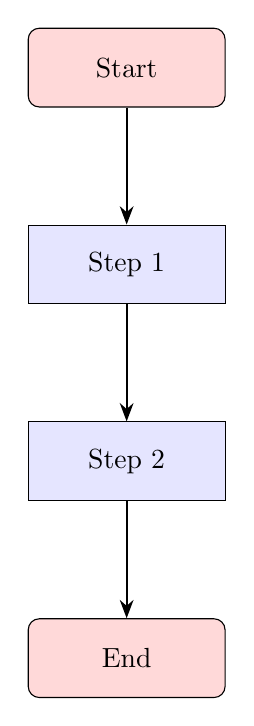
\begin{tikzpicture}[node distance=2.5cm]
    \node (start) [startstop] {Start};
    \node (step1) [process, below of=start] {Step 1};
    \node (step2) [process, below of=step1] {Step 2};
    \node (end)   [startstop, below of=step2] {End};
    
    \draw [arrow] (start) -- (step1);
    \draw [arrow] (step1) -- (step2);
    \draw [arrow] (step2) -- (end);
\end{tikzpicture}
\end{center}

\subsection{2. Workflow Diagram}
Focuses on human-centric tasks and office routines.
\begin{center}
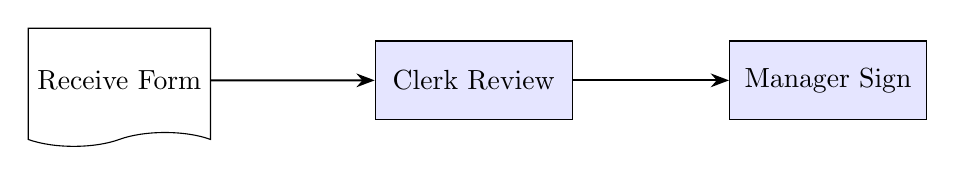
\begin{tikzpicture}[node distance=2.5cm]
    \node (doc)     [doc] {Receive Form};
    \node (clerk)   [process, right of=doc, xshift=2cm] {Clerk Review};
    \node (manager) [process, right of=clerk, xshift=2cm] {Manager Sign};
    \draw [arrow] (doc) -- (clerk);
    \draw [arrow] (clerk) -- (manager);
\end{tikzpicture}
\end{center}

\subsection{3. Swimlane (Cross-Functional) Diagram}
\begin{center}
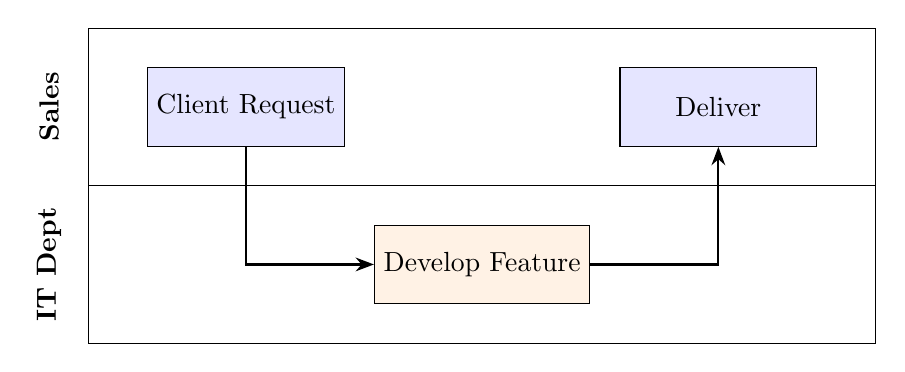
\begin{tikzpicture}
    \draw (0,0) rectangle (10,-4);
    \draw (0,-2) -- (10,-2);
    \node[rotate=90, font=\bfseries] at (-0.5,-1) {Sales};
    \node[rotate=90, font=\bfseries] at (-0.5,-3) {IT Dept};
    
    \node (req) [process] at (2,-1) {Client Request};
    \node (dev) [process, fill=orange!10] at (5,-3) {Develop Feature};
    \node (del) [process] at (8,-1) {Deliver};
    
    \draw [arrow] (req) |- (dev);
    \draw [arrow] (dev) -| (del);
\end{tikzpicture}
\end{center}

\subsection{4. Value Stream Map (VSM)}
% Fixed: use .south/.north anchors to make the material flow direction unambiguous.
\begin{center}
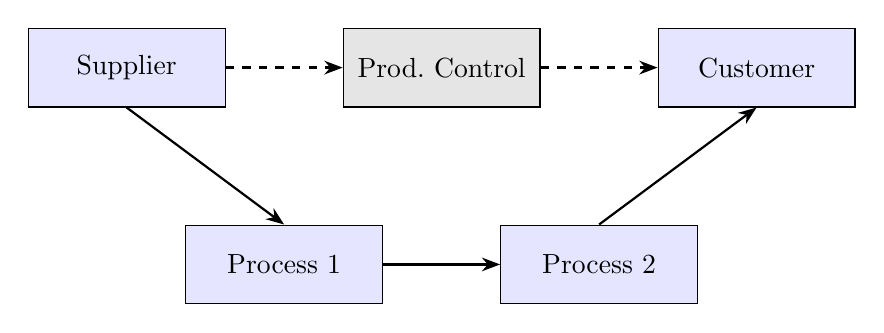
\begin{tikzpicture}
    % Top row: information flow
    \node (supplier) [process] at (0,2.5)   {Supplier};
    \node (prodCtrl) [process, fill=gray!20] at (4,2.5) {Prod.\ Control};
    \node (customer) [process] at (8,2.5)   {Customer};
    % Bottom row: material flow
    \node (manuf1)   [process] at (2,0)     {Process 1};
    \node (manuf2)   [process] at (6,0)     {Process 2};
    % Information flow (dashed, top)
    \draw [->, dashed, thick, >=Stealth] (supplier) -- (prodCtrl);
    \draw [->, dashed, thick, >=Stealth] (prodCtrl) -- (customer);
    % Material flow: straight vertical then horizontal, direction always clear
    \draw [arrow] (supplier.south) -- (manuf1.north);
    \draw [arrow] (manuf1)         -- (manuf2);
    \draw [arrow] (manuf2.north)   -- (customer.south);
\end{tikzpicture}
\end{center}

\subsection{5. EPC (Event-driven Process Chain)}
Hexagons for events, rounded rectangles for functions.
\begin{center}
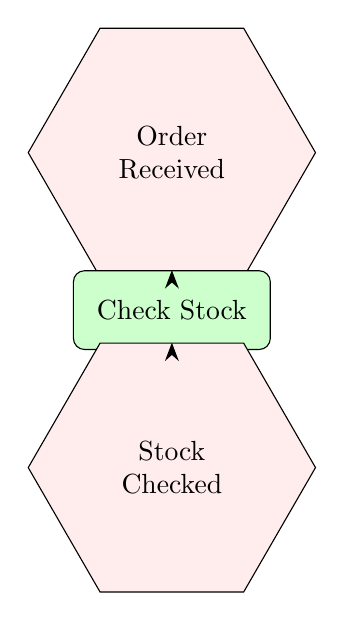
\begin{tikzpicture}[node distance=2cm]
    \node (event1) [regular polygon, regular polygon sides=6, draw, fill=pink!30,
                    text width=2cm, align=center] {Order\\Received};
    \node (func)   [process, rounded corners, below of=event1, fill=green!20] {Check Stock};
    \node (event2) [regular polygon, regular polygon sides=6, draw, fill=pink!30,
                    below of=func, text width=2cm, align=center] {Stock\\Checked};
    
    \draw [arrow] (event1) -- (func);
    \draw [arrow] (func)   -- (event2);
\end{tikzpicture}
\end{center}

\subsection{6. BPMN (Business Process Model and Notation) Diagram}
Circles for start/end events, diamonds for exclusive gateways.
\begin{center}
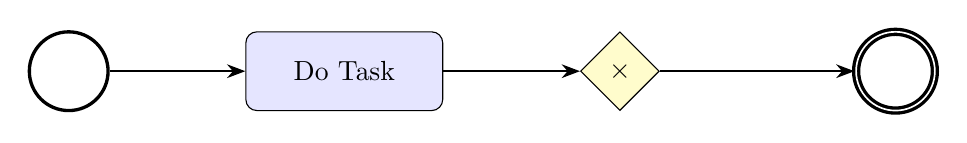
\begin{tikzpicture}[node distance=2.5cm]
    \node (start)   [circle, draw, very thick, minimum size=1cm] {};
    \node (task)    [process, rounded corners, right of=start, xshift=1cm] {Do Task};
    \node (gateway) [diamond, draw, fill=yellow!20, right of=task, xshift=1cm,
                     inner sep=0pt, minimum size=1cm] {$\times$};
    \node (end)     [circle, draw, very thick, double, right of=gateway,
                     xshift=1cm, minimum size=1cm] {};
    
    \draw [arrow] (start)   -- (task);
    \draw [arrow] (task)    -- (gateway);
    \draw [arrow] (gateway) -- (end);
\end{tikzpicture}
\end{center}

\subsection{7. SIPOC (Supplier, Input, Process, Output, Customer) Diagram}
Best represented as a structured table using \texttt{tabularx} and \texttt{booktabs}.
\begin{center}
\begin{tabularx}{\textwidth}{@{}XXXXX@{}}
    \toprule
    \textbf{Supplier} & \textbf{Input} & \textbf{Process} & \textbf{Output} & \textbf{Customer} \\
    \midrule
    Vendor & Raw Materials & Manufacturing & Finished Goods & Retailer \\
    \bottomrule
\end{tabularx}
\end{center}

% ============================================================
\section{Software, Tech \& Data Flowcharts}
% ============================================================

% Fixed: use 'near start' to prevent the label overlapping the process circle.
\begin{center}
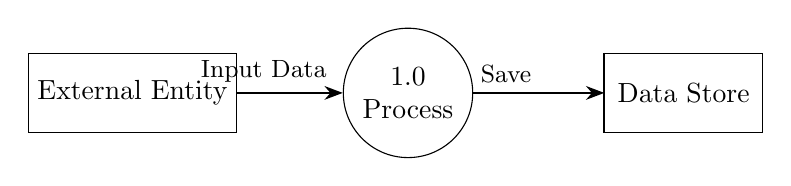
\begin{tikzpicture}[node distance=3.5cm]
    \node (ext)   [draw, rectangle, minimum height=1cm, minimum width=2.2cm] {External Entity};
    \node (proc)  [draw, circle, right of=ext, align=center, minimum size=1.5cm] {1.0\\Process};
    \node (store) [draw, rectangle, right of=proc,
                   minimum height=1cm, minimum width=2cm] {Data Store};
    % Data store double-line decoration
    \draw[thick] (store.north west) -- (store.south west);

    \draw [arrow] (ext)  -- node[above, near start]{\small Input Data} (proc);
    \draw [arrow] (proc) -- node[above, near start]{\small Save}       (store);
\end{tikzpicture}
\end{center}

\subsection{9. System Flowchart}
Shows hardware/network data movement.
\begin{center}
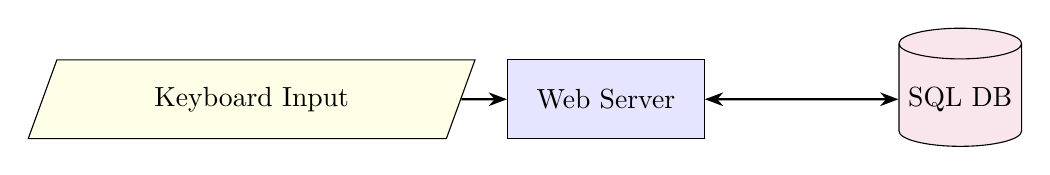
\begin{tikzpicture}[node distance=2.5cm]
    \node (input)  [io]                              {Keyboard Input};
    \node (server) [process, right of=input, xshift=2cm] {Web Server};
    \node (db)     [database, right of=server, xshift=2cm] {SQL DB};
    
    \draw [arrow] (input) -- (server);
    \draw [<->, thick, >=Stealth] (server) -- (db);
\end{tikzpicture}
\end{center}

\subsection{10. Program Flowchart}
\begin{center}
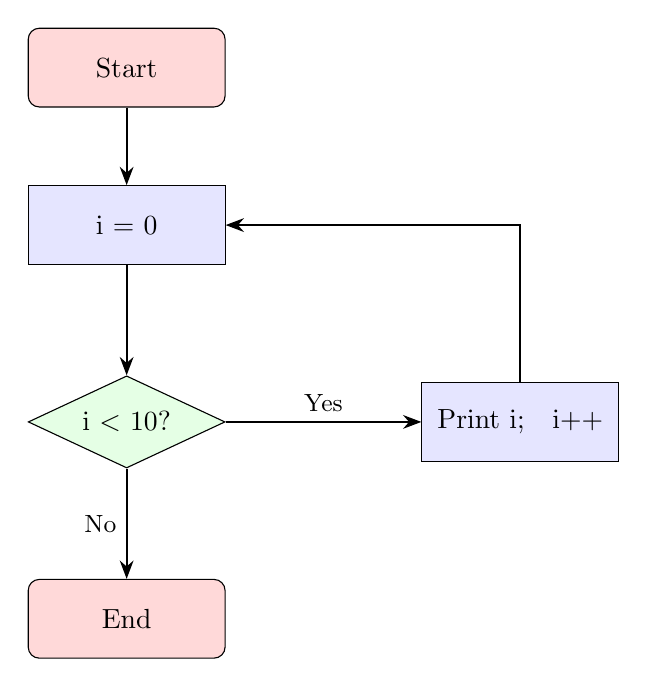
\begin{tikzpicture}[node distance=2cm]
    \node (start) [startstop] {Start};
    \node (init)  [process, below of=start] {i = 0};
    \node (cond)  [decision, below of=init, yshift=-0.5cm] {i $<$ 10?};
    \node (loop)  [process, right of=cond, xshift=3cm] {Print i;\quad i++};
    \node (end)   [startstop, below of=cond, yshift=-0.5cm] {End};
    
    \draw [arrow] (start) -- (init);
    \draw [arrow] (init)  -- (cond);
    \draw [arrow] (cond)  -- node[anchor=south] {\small Yes} (loop);
    \draw [arrow] (loop)  |- (init);
    \draw [arrow] (cond)  -- node[anchor=east]  {\small No}  (end);
\end{tikzpicture}
\end{center}

\subsection{11. SDL (Specification and Description Language) Diagram}
Standardized shapes for telecommunications and software behavior.
\begin{center}
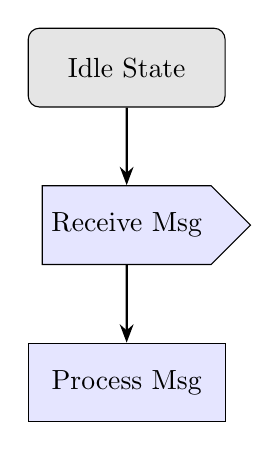
\begin{tikzpicture}[node distance=2cm]
    \node (state)  [process, rounded corners, fill=gray!20] {Idle State};
    \node (signal) [draw, signal, signal to=east, below of=state,
                    fill=blue!10, minimum width=2.5cm, minimum height=1cm,
                    text centered] {Receive Msg};
    \node (task)   [process, below of=signal] {Process Msg};
    
    \draw [arrow] (state)  -- (signal);
    \draw [arrow] (signal) -- (task);
\end{tikzpicture}
\end{center}

\subsection{12. UML (Unified Modeling Language) Activity Diagram}
Shows dynamic execution behavior.
\begin{center}
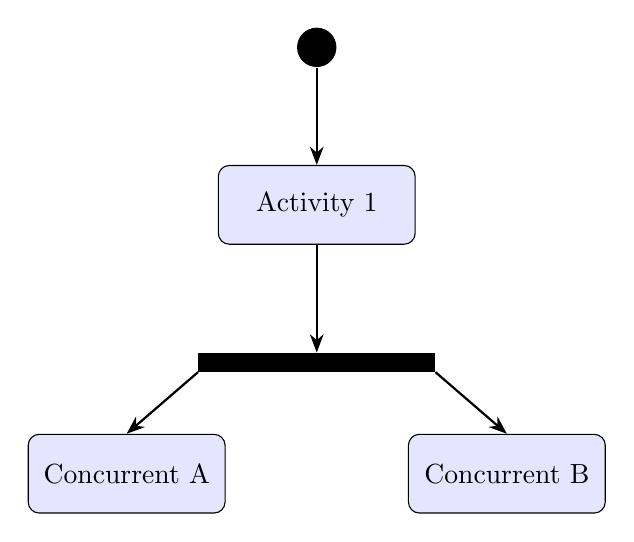
\begin{tikzpicture}[node distance=2cm]
    \node (start) [circle, fill=black, minimum size=0.5cm] {};
    \node (act1)  [process, rounded corners, below of=start] {Activity 1};
    \node (fork)  [draw, fill=black, minimum width=3cm, minimum height=0.2cm,
                   below of=act1] {};
    \node (act2)  [process, rounded corners, below left of=fork,  xshift=-1cm] {Concurrent A};
    \node (act3)  [process, rounded corners, below right of=fork, xshift=1cm]  {Concurrent B};
    
    \draw [arrow] (start)          -- (act1);
    \draw [arrow] (act1)           -- (fork);
    \draw [arrow] (fork.south west) -- (act2.north);
    \draw [arrow] (fork.south east) -- (act3.north);
\end{tikzpicture}
\end{center}

% ============================================================
\section{Logic, Strategy \& Troubleshooting Flowcharts}
% ============================================================

\subsection{13. Decision Tree Diagram}
\begin{center}
\begin{forest}
  for tree={draw, align=center, edge={thick, -Stealth},
            minimum width=2cm, minimum height=0.8cm, s sep=1.5cm}
  [Is it raining?
    [Yes [Stay Inside]]
    [No  [Go for a Walk]]
  ]
\end{forest}
\end{center}

\subsection{14. Troubleshooting Flowchart}
\begin{center}
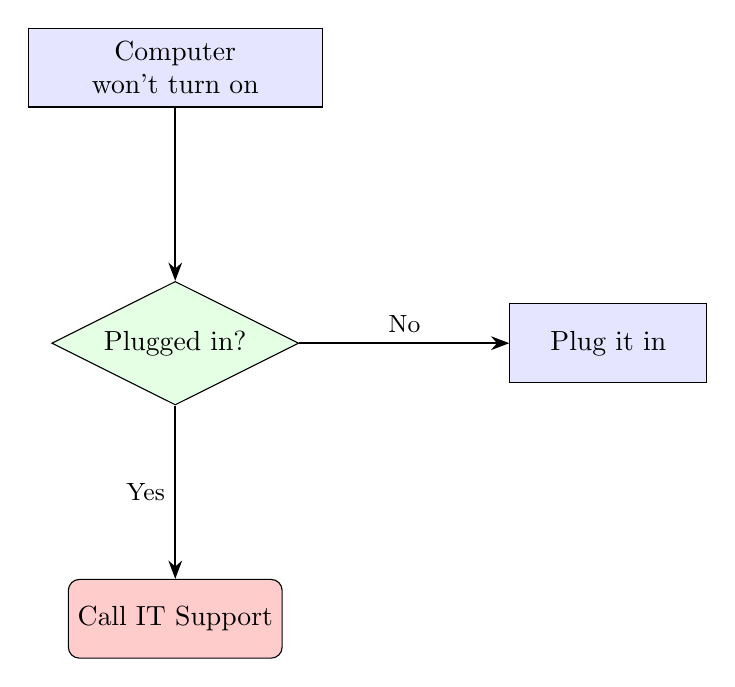
\begin{tikzpicture}[node distance=2.5cm]
    \node (prob)   [process, text width=3.5cm] {Computer won't turn on};
    \node (dec)    [decision, below of=prob, yshift=-1cm] {Plugged in?};
    \node (plug)   [process, right of=dec, xshift=3cm] {Plug it in};
    \node (broken) [startstop, fill=red!20, below of=dec, yshift=-1cm] {Call IT Support};
    
    \draw [arrow] (prob)   -- (dec);
    \draw [arrow] (dec)    -- node[anchor=south] {\small No}  (plug);
    \draw [arrow] (dec)    -- node[anchor=east]  {\small Yes} (broken);
\end{tikzpicture}
\end{center}

\subsection{15. Fishbone (Ishikawa) Diagram}
\begin{center}
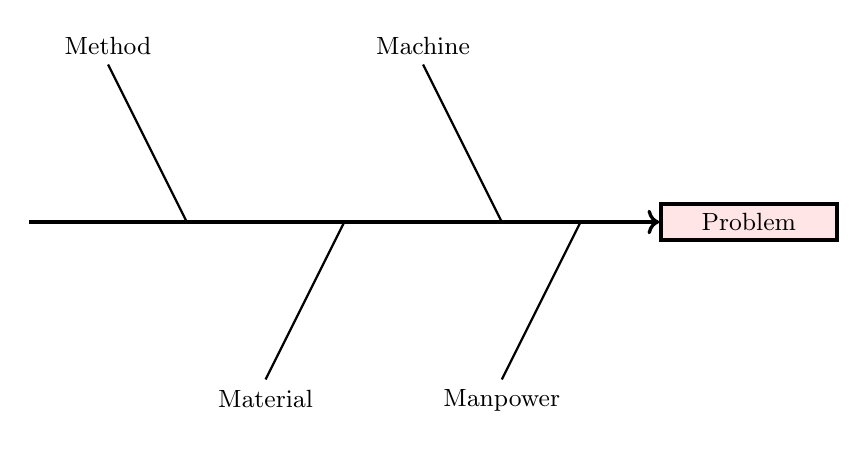
\begin{tikzpicture}[font=\small]
    \draw[very thick, ->] (0,0) -- (8,0)
        node[right, draw, fill=red!10, text width=2cm, align=center] {Problem};
    \draw[thick] (2,0) -- (1,2)   node[above] {Method};
    \draw[thick] (6,0) -- (5,2)   node[above] {Machine};
    \draw[thick] (4,0) -- (3,-2)  node[below] {Material};
    \draw[thick] (7,0) -- (6,-2)  node[below] {Manpower};
\end{tikzpicture}
\end{center}

\subsection{16. PERT (Program Evaluation and Review Technique) Chart}
Used in project management to show task dependencies.
\begin{center}
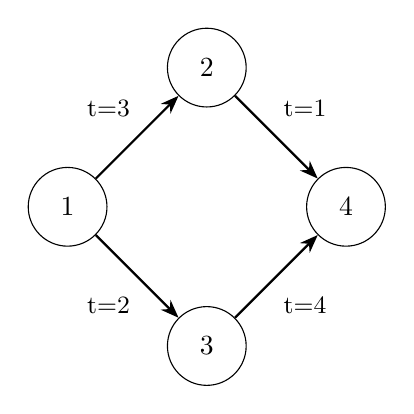
\begin{tikzpicture}[node distance=2.5cm,
    every node/.style={circle, draw, minimum size=1cm}]
    \node (n1) {1};
    \node (n2) [above right of=n1] {2};
    \node (n3) [below right of=n1] {3};
    \node (n4) [below right of=n2] {4};
    
    \draw [arrow] (n1) -- node[draw=none, above left]  {\small t=3} (n2);
    \draw [arrow] (n1) -- node[draw=none, below left]  {\small t=2} (n3);
    \draw [arrow] (n2) -- node[draw=none, above right] {\small t=1} (n4);
    \draw [arrow] (n3) -- node[draw=none, below right] {\small t=4} (n4);
\end{tikzpicture}
\end{center}

% ============================================================
\section{Comparison \& Relationship Diagrams}
% ============================================================

\subsection{17. Venn Diagram}
% Note: blend group=multiply requires transparency and slows compilation.
% Using opacity instead for fast rendering.
\begin{center}
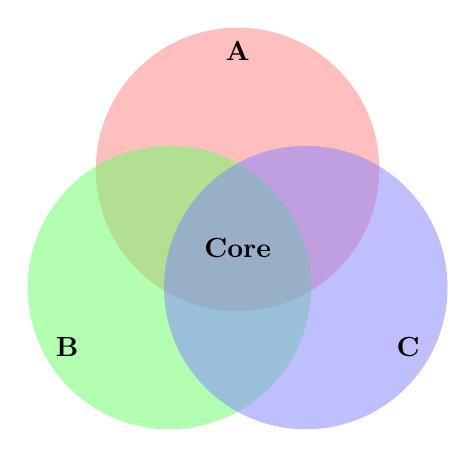
\begin{tikzpicture}
    \fill[red!50, opacity=0.5]   ( 90:1.0) circle (1.8);
    \fill[green!60, opacity=0.5] (210:1.0) circle (1.8);
    \fill[blue!50, opacity=0.5]  (330:1.0) circle (1.8);
    \node at ( 90:2.5) {\textbf{A}};
    \node at (210:2.5) {\textbf{B}};
    \node at (330:2.5) {\textbf{C}};
    \node [font=\bfseries] at (0,0) {Core};
\end{tikzpicture}
\end{center}

\subsection{18. Mind Map}
% Note: The mindmap TikZ library is very slow (~5-8s alone).
% This uses the fast `trees` library to produce an equivalent visual.
\begin{center}
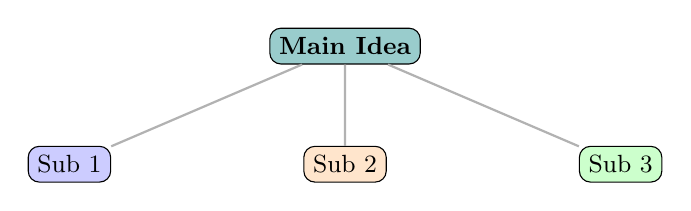
\begin{tikzpicture}[
    every node/.style={rounded corners, draw, align=center, font=\small},
    level 1/.style={sibling distance=3.5cm, fill=teal!20},
    level 2/.style={sibling distance=2cm, fill=teal!10},
    edge from parent/.style={thick, draw=gray!60}
]
\node[fill=teal!40, font=\bfseries\small] {Main Idea}
    child { node[fill=blue!20]   {Sub 1} }
    child { node[fill=orange!20] {Sub 2} }
    child { node[fill=green!20]  {Sub 3} };
\end{tikzpicture}
\end{center}

\subsection{19. Matrix Diagram (BCG/SWOT Grid)}
(BCG = Boston Consulting Group; SWOT = Strengths, Weaknesses, Opportunities, Threats)
A 2x2 grid is easiest to implement using a simple \texttt{tikzpicture} with explicit coordinates.
\begin{center}
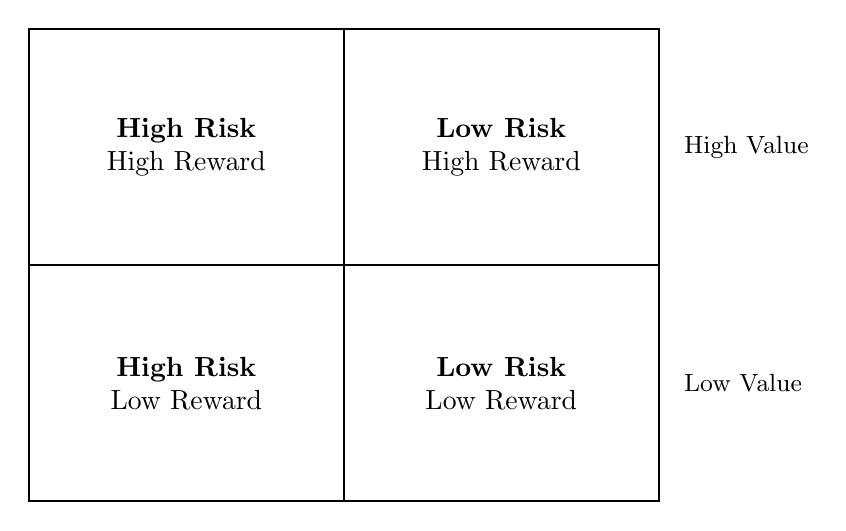
\begin{tikzpicture}
    \draw[thick] (0,0) rectangle (8,6);
    \draw[thick] (0,3) -- (8,3);
    \draw[thick] (4,0) -- (4,6);
    
    \node[align=center] at (2,4.5) {\textbf{High Risk}\\High Reward};
    \node[align=center] at (6,4.5) {\textbf{Low Risk}\\High Reward};
    \node[align=center] at (2,1.5) {\textbf{High Risk}\\Low Reward};
    \node[align=center] at (6,1.5) {\textbf{Low Risk}\\Low Reward};
    
    \node[anchor=west] at (8.2, 4.5) {\small High Value};
    \node[anchor=west] at (8.2, 1.5) {\small Low Value};
\end{tikzpicture}
\end{center}

\subsection{20. Scatter Plot (using \texttt{pgfplots})}
\begin{center}
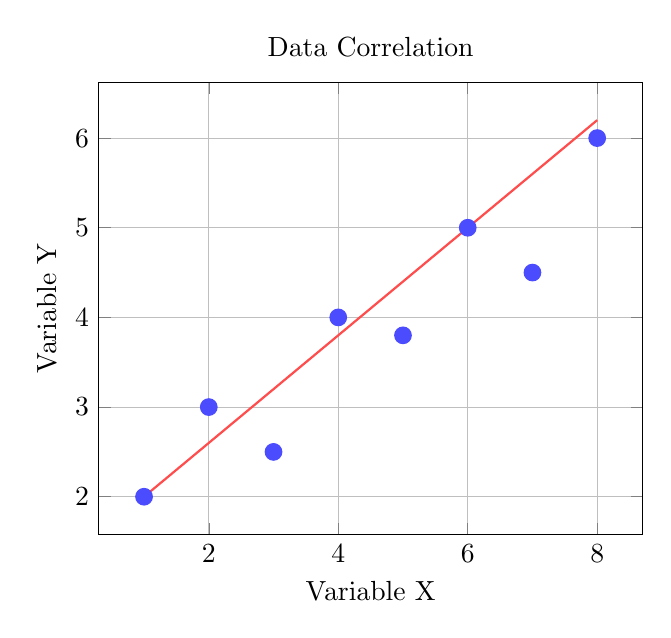
\begin{tikzpicture}
\begin{axis}[title={Data Correlation}, xlabel={Variable X}, ylabel={Variable Y},
             grid=major, width=0.7\textwidth]
    \addplot[only marks, mark=*, blue!70, mark size=3pt] coordinates {
        (1,2) (2,3) (3,2.5) (4,4) (5,3.8) (6,5) (7,4.5) (8,6)
    };
    \addplot[thick, red!70, domain=1:8] {0.6*x + 1.4};
\end{axis}
\end{tikzpicture}
\end{center}

\subsection{21. Bubble Chart (using \texttt{pgfplots})}
\begin{center}
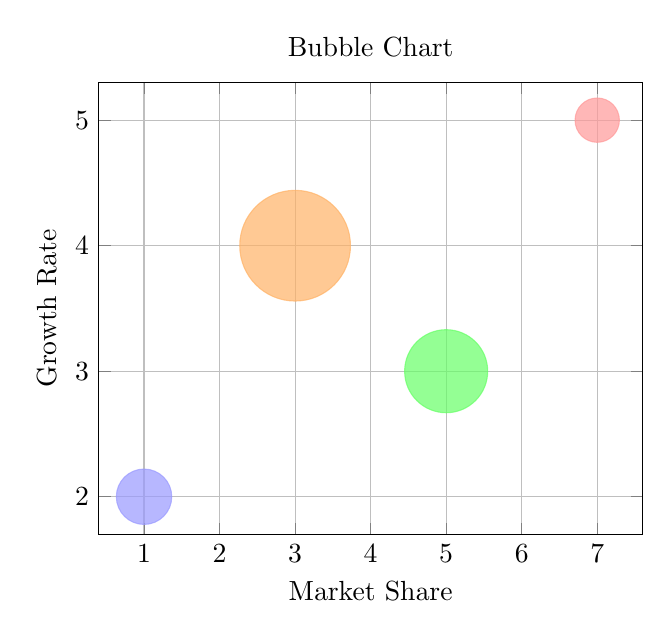
\begin{tikzpicture}
\begin{axis}[title={Bubble Chart}, xlabel={Market Share}, ylabel={Growth Rate},
             grid=major, width=0.7\textwidth]
    % Simulate bubbles using mark size to represent a 3rd variable
    \addplot[only marks, mark=*, mark size=10pt, blue!40!white,  opacity=0.7] coordinates {(1, 2)};
    \addplot[only marks, mark=*, mark size=20pt, orange!60!white, opacity=0.7] coordinates {(3, 4)};
    \addplot[only marks, mark=*, mark size=15pt, green!60!white,  opacity=0.7] coordinates {(5, 3)};
    \addplot[only marks, mark=*, mark size=8pt,  red!40!white,    opacity=0.7] coordinates {(7, 5)};
\end{axis}
\end{tikzpicture}
\end{center}

% ============================================================
\section{Structured Business \& Project Diagrams}
% ============================================================

\subsection{22. Organizational Chart}
\begin{center}
\begin{forest}
  for tree={draw, align=center, fill=blue!5, rounded corners,
            edge={thick, -Stealth}, s sep=1cm, l sep=1.5cm}
  [CEO
    [VP Eng [Team A] [Team B]]
    [VP Sales [Region A]]
    [VP HR]
  ]
\end{forest}
\end{center}

\subsection{23. Gantt Chart}
\begin{center}
\begin{ganttchart}[vgrid, hgrid,
    bar/.style={fill=blue!50},
    bar label font=\small,
    title label font=\small\bfseries,
    y unit chart=0.7cm]{1}{12}
  \gantttitle{Project Timeline (Weeks)}{12} \\
  \gantttitlelist{1,...,12}{1} \\
  \ganttbar{Planning}{1}{2} \\
  \ganttlinkedbar{Design}{3}{5} \\
  \ganttlinkedbar{Development}{6}{10} \\
  \ganttlinkedbar{Testing}{11}{12}
\end{ganttchart}
\end{center}

\subsection{24. Funnel Chart}
\begin{center}
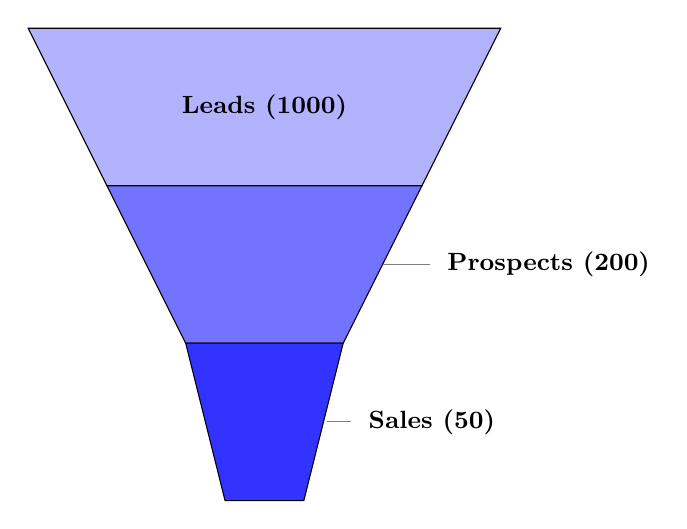
\begin{tikzpicture}
    % Top tier -- widest, so label fits fine inside
    \draw[fill=blue!30] (-3,4) -- (3,4) -- (2,2) -- (-2,2) -- cycle;
    \node[font=\small\bfseries] at (0,3) {Leads (1000)};

    % Middle tier -- label placed to the RIGHT to avoid clipping
    \draw[fill=blue!55] (-2,2) -- (2,2) -- (1,0) -- (-1,0) -- cycle;
    \node[anchor=west, font=\small\bfseries] at (2.2,1) {Prospects (200)};
    \draw[gray, thin] (1.5,1) -- (2.1,1);

    % Bottom tier -- label placed to the RIGHT
    \draw[fill=blue!80] (-1,0) -- (1,0) -- (0.5,-2) -- (-0.5,-2) -- cycle;
    \node[anchor=west, font=\small\bfseries] at (1.2,-1) {Sales (50)};
    \draw[gray, thin] (0.8,-1) -- (1.1,-1);
\end{tikzpicture}
\end{center}

% ============================================================
\section{Technical \& System Diagrams}
% ============================================================

\subsection{25. Network Diagram}
\begin{center}
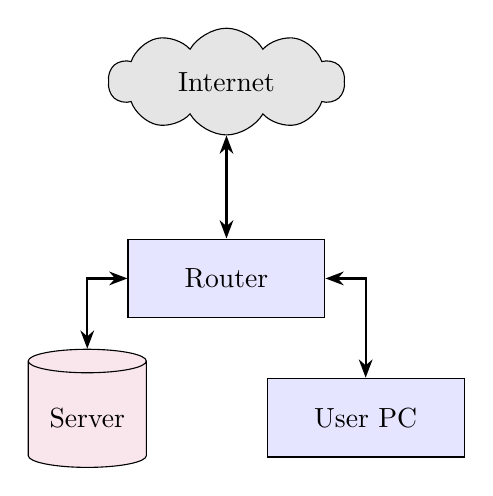
\begin{tikzpicture}[node distance=2.5cm]
    \node (internet) [draw, cloud, cloud puffs=10, cloud puff arc=120,
                      aspect=2, fill=gray!20, minimum width=3cm] {Internet};
    \node (router)   [process, below of=internet, fill=blue!10] {Router};
    \node (server)   [database, below left of=router, fill=purple!10] {Server};
    \node (pc)       [process, below right of=router] {User PC};
    
    \draw [<->, thick, >=Stealth] (internet) -- (router);
    \draw [<->, thick, >=Stealth] (router)   -| (server);
    \draw [<->, thick, >=Stealth] (router)   -| (pc);
\end{tikzpicture}
\end{center}

\subsection{26. Entity-Relationship Diagram (ERD)}
\begin{center}
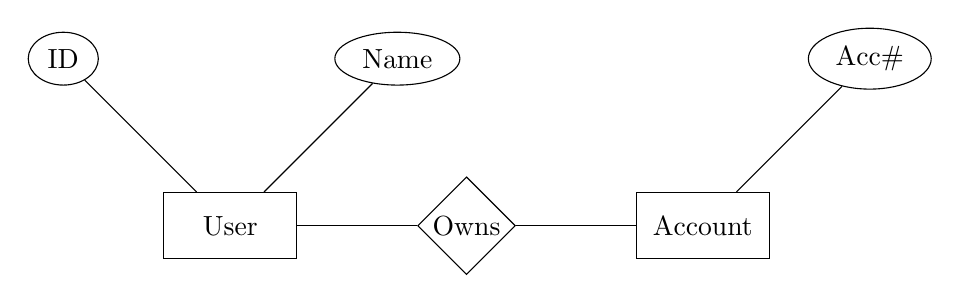
\begin{tikzpicture}[node distance=3cm]
    \node[entity] (user)    {User};
    \node[attribute] (uid)  [above left of=user]  {\key{ID}}     edge (user);
    \node[attribute] (name) [above right of=user] {Name}         edge (user);
    \node[relationship] (owns) [right of=user] {Owns}            edge (user);
    \node[entity] (account) [right of=owns]    {Account}         edge (owns);
    \node[attribute] (accid) [above right of=account] {\key{Acc\#}} edge (account);
\end{tikzpicture}
\end{center}

\subsection{27. UML (Unified Modeling Language) Class Diagram}
Using the \texttt{shapes.multipart} library to create split rectangles for attributes/methods.
\begin{center}
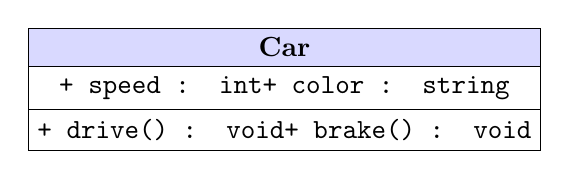
\begin{tikzpicture}
    \node[draw, rectangle split, rectangle split parts=3,
          rectangle split part fill={blue!15, white, white},
          minimum width=4.5cm] (class) {
        \textbf{Car}
        \nodepart{two}
        \texttt{+ speed : int}\par
        \texttt{+ color : string}
        \nodepart{three}
        \texttt{+ drive() : void}\par
        \texttt{+ brake() : void}
    };
\end{tikzpicture}
\end{center}

\subsection{28. Circuit Schematic}
\begin{center}
\begin{circuitikz}
    \draw (0,0)
        to[battery, l=$9\,\mathrm{V}$] (0,3)
        to[switch, l=S1]               (3,3)
        to[R, l=$100\,\Omega$]         (3,1.5)
        to[led, l=LED]                 (3,0)
        -- (0,0);
\end{circuitikz}
\end{center}

% ============================================================
\section{Additional Diagram Types}
% ============================================================

\subsection{29. UML (Unified Modeling Language) Sequence Diagram}
Models the time-ordered interaction between objects or services.
\begin{center}
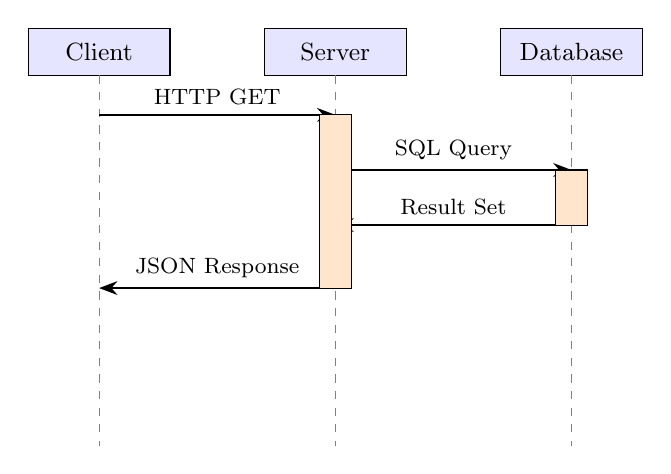
\begin{tikzpicture}[font=\small]
    % Lifelines
    \foreach \x/\name in {0/Client, 3/Server, 6/Database} {
        \node[draw, fill=blue!10, minimum width=1.8cm, minimum height=0.6cm]
            at (\x, 0) {\name};
        \draw[dashed, gray] (\x,-0.3) -- (\x,-5);
    }
    % Messages (horizontal arrows)
    \draw[arrow] (0,-0.8) -- node[above]{\footnotesize HTTP GET} (3,-0.8);
    \draw[arrow] (3,-1.5) -- node[above]{\footnotesize SQL Query} (6,-1.5);
    \draw[arrow] (6,-2.2) -- node[above]{\footnotesize Result Set} (3,-2.2);
    \draw[arrow] (3,-3.0) -- node[above]{\footnotesize JSON Response} (0,-3.0);
    % Activation boxes
    \draw[fill=orange!20] (2.8,-0.8) rectangle (3.2,-3.0);
    \draw[fill=orange!20] (5.8,-1.5) rectangle (6.2,-2.2);
\end{tikzpicture}
\end{center}

\subsection{30. State Machine Diagram}
Models system states and the events that trigger transitions.
\begin{center}
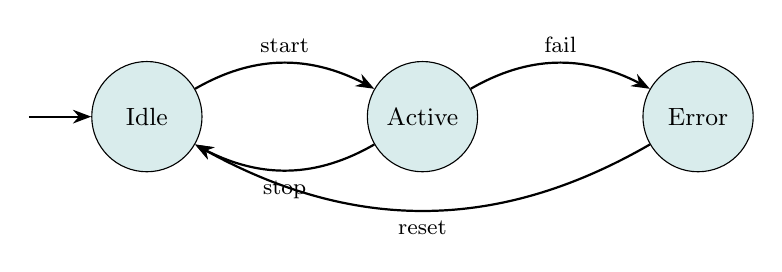
\begin{tikzpicture}[node distance=3.5cm,
    state/.style={circle, draw, fill=teal!15, minimum size=1.4cm, font=\small}]
    \node[state] (idle)    {Idle};
    \node[state, right of=idle]    (active)  {Active};
    \node[state, right of=active]  (error)   {Error};

    \draw[arrow] (-1.5,0) -- (idle);
    \draw[arrow, bend left=30] (idle)   to node[above]{\footnotesize start}  (active);
    \draw[arrow, bend left=30] (active) to node[below]{\footnotesize stop}   (idle);
    \draw[arrow, bend left=30] (active) to node[above]{\footnotesize fail}   (error);
    \draw[arrow, bend left=30] (error)  to node[below]{\footnotesize reset}  (idle);
\end{tikzpicture}
\end{center}

\subsection{31. Timeline Diagram}
A linear representation of milestones on a time axis.
% Fixed: ifthenelse with string comparison is invalid in pgfmath.
% Each milestone is an explicit node to correctly alternate above/below.
\begin{center}
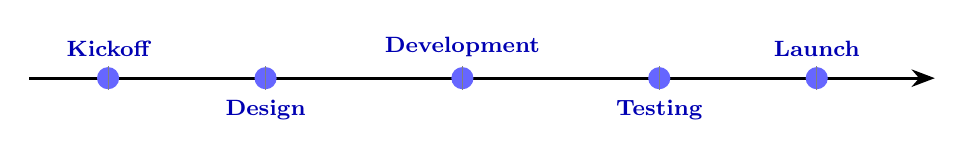
\begin{tikzpicture}[font=\small]
    \draw[very thick, ->, >=Stealth] (0,0) -- (11.5,0);
    % Tick marks
    \foreach \x in {1, 3, 5.5, 8, 10} {
        \fill[blue!60] (\x,0) circle (4pt);
        \draw[gray, thin] (\x,0.15) -- (\x,-0.15);
    }
    % Labels alternating above and below manually
    \node[above, font=\footnotesize\bfseries, text=blue!70!black] at (1,   0.15) {Kickoff};
    \node[below, font=\footnotesize\bfseries, text=blue!70!black] at (3,  -0.15) {Design};
    \node[above, font=\footnotesize\bfseries, text=blue!70!black] at (5.5, 0.15) {Development};
    \node[below, font=\footnotesize\bfseries, text=blue!70!black] at (8,  -0.15) {Testing};
    \node[above, font=\footnotesize\bfseries, text=blue!70!black] at (10,  0.15) {Launch};
\end{tikzpicture}
\end{center}

\subsection{32. Data Pipeline Diagram}
Shows the flow of data between processing stages (ETL-style).
\begin{center}
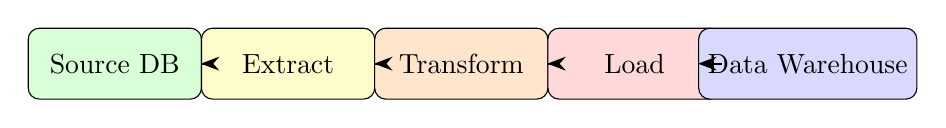
\begin{tikzpicture}[node distance=2.2cm,
    pipe/.style={rectangle, rounded corners=4pt, minimum width=2.2cm,
                 minimum height=0.9cm, text centered, draw=black}]
    \node[pipe, fill=green!15]  (src)    {Source DB};
    \node[pipe, fill=yellow!20, right of=src]  (ext)  {Extract};
    \node[pipe, fill=orange!20, right of=ext]  (trn)  {Transform};
    \node[pipe, fill=red!15,    right of=trn]  (load) {Load};
    \node[pipe, fill=blue!15,   right of=load] (dw)   {Data Warehouse};

    \draw[arrow] (src) -- (ext);
    \draw[arrow] (ext) -- (trn);
    \draw[arrow] (trn) -- (load);
    \draw[arrow] (load) -- (dw);
\end{tikzpicture}
\end{center}

\subsection{33. Radar / Spider Chart (using pgfplots)}
Compares multiple variables on axes radiating from the same centre.
\begin{center}
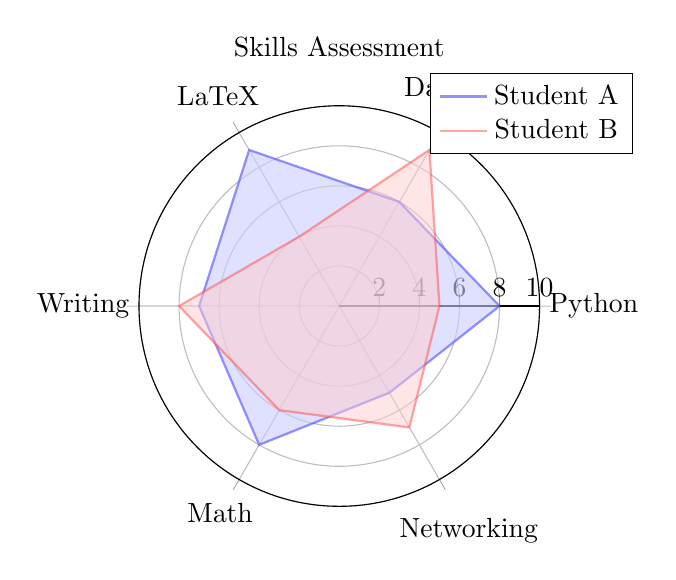
\begin{tikzpicture}
\begin{polaraxis}[
    title={Skills Assessment},
    xtick={0,60,120,180,240,300},
    xticklabels={Python, Databases, LaTeX, Writing, Math, Networking},
    ymin=0, ymax=10,
    ytick={2,4,6,8,10},
    width=0.55\textwidth
]
    \addplot[thick, blue!70, fill=blue!20, opacity=0.6]
        coordinates {(0,8) (60,6) (120,9) (180,7) (240,8) (300,5) (360,8)};
    \addplot[thick, red!70, fill=red!20, opacity=0.5]
        coordinates {(0,5) (60,9) (120,4) (180,8) (240,6) (300,7) (360,5)};
    \legend{Student A, Student B}
\end{polaraxis}
\end{tikzpicture}
\end{center}

\subsection{34. Layered Architecture Diagram}
Represents software layers (Presentation, Logic, Data) stacked vertically.
% Fixed: \foreach with '!' in color names causes token split errors.
% Each layer is drawn explicitly instead.
\begin{center}
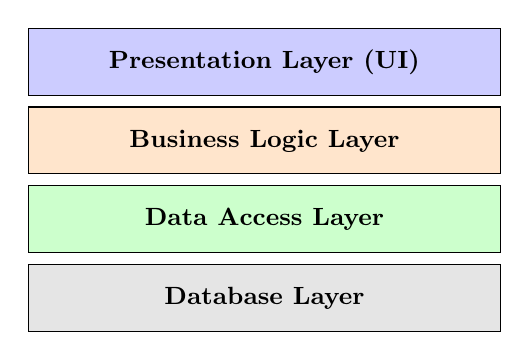
\begin{tikzpicture}[font=\small]
    \draw[fill=blue!20,   draw=black] (-3,3) rectangle (3,3.85);
    \node at (0,3.42) {\textbf{Presentation Layer (UI)}};

    \draw[fill=orange!20, draw=black] (-3,2) rectangle (3,2.85);
    \node at (0,2.42) {\textbf{Business Logic Layer}};

    \draw[fill=green!20,  draw=black] (-3,1) rectangle (3,1.85);
    \node at (0,1.42) {\textbf{Data Access Layer}};

    \draw[fill=gray!20,   draw=black] (-3,0) rectangle (3,0.85);
    \node at (0,0.42) {\textbf{Database Layer}};
\end{tikzpicture}
\end{center}

\subsection{35. Comparison Table (Feature Matrix)}
A structured matrix comparing products or options across features.
\begin{center}
\begin{tabular}{lccc}
    \toprule
    \textbf{Feature} & \textbf{Basic} & \textbf{Pro} & \textbf{Enterprise} \\
    \midrule
    Collaboration     & $\times$ & $\checkmark$ & $\checkmark$ \\
    Version History   & $\times$ & $\checkmark$ & $\checkmark$ \\
    GitHub Sync       & $\times$ & $\times$     & $\checkmark$ \\
    Custom Templates  & $\times$ & $\checkmark$ & $\checkmark$ \\
    Priority Support  & $\times$ & $\times$     & $\checkmark$ \\
    \bottomrule
\end{tabular}
\end{center}

\end{document}
